\chapter{Genome assembly of Candida nivariensis}
\label{chap:nivar}





This document was generated on Mon May  2 22:40:12 2022.

As shown in Figure \ref{fig:mummer} and in Table \ref{tab:rtab1} we can see that bla bla \citep{B}.


\begin{figure}[!ht]
\centering
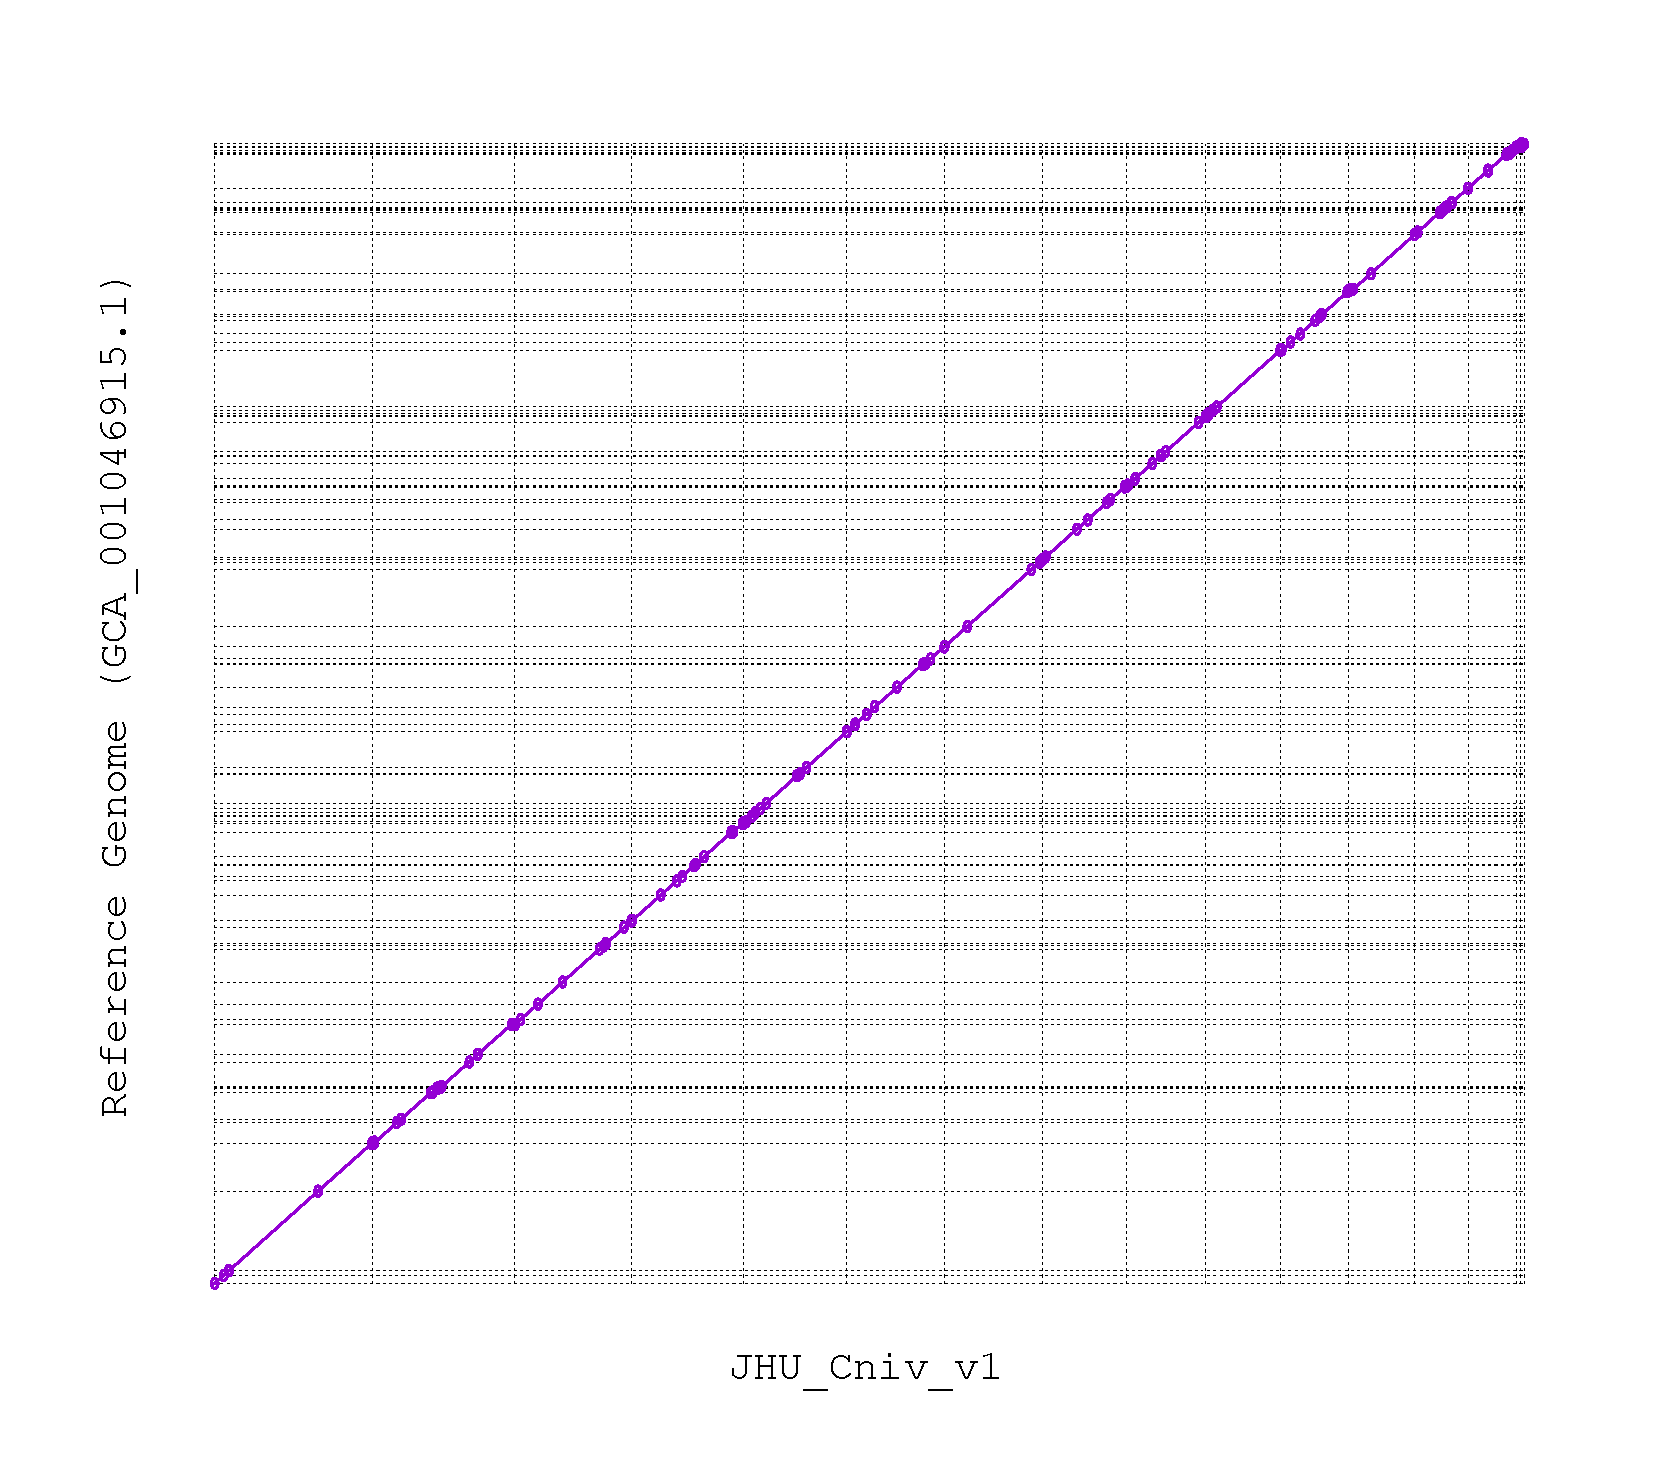
\includegraphics[width = 1\linewidth,keepaspectratio]{figure/mummer.pdf}
\caption[Mummer between stuff]{{\bf Mummer between stuff.} {\bf (a)} blah first point {\bf (b)} blah second point {\bf (c)} blaih thrid panel  }
\label{fig:mummer}
\end{figure}




% latex table generated in R 4.2.0 by xtable 1.8-4 package
% Mon May  2 22:40:12 2022
\begin{table}[ht]
\centering
\begin{tabular}{rr}
  \hline
A & B \\ 
  \hline
  1 & 1.88 \\ 
    2 & -1.42 \\ 
    3 & -0.01 \\ 
    4 & -0.85 \\ 
    5 & 0.82 \\ 
    6 & -0.03 \\ 
    7 & -0.56 \\ 
    8 & 0.96 \\ 
    9 & 0.03 \\ 
   10 & 0.36 \\ 
   \hline
\end{tabular}
\caption{\bf{ Table title } Table description} 
\label{tab:rtab1}
\end{table}

